\chapter{Theoretical background} \label{chr:theory}

\section{Radiation therapy}

\emph{Radiation therapy} is a treatment that utilizes beams of ionising radiation to control the growth or kill cancer cells. This type of treatment can be effective in cases where the cancerous cells are concentrated in a particular area of the body and have not spread to other regions. This treatment requires specialised, high-precision equipment - \emph{linear particle accelerators}. \cite{abeloff_clinical_oncology}

\subsection{Linear particle accelerator}

A linear particle accelerator, often referred to as a \emph{linac}, is a device that accelerates charged particles (electrons) to velocities near the speed of light by using oscillating electric fields to push the electrons through a series of accelerating cavities. Subsequently, these electrons collide with a heavy metal target, resulting in the generation of high-energy X-rays. These are then shaped as required upon exiting the machine. \cite{how_linac_work}

\subsubsection{Linac rotation and isocenter}

Linear accelerators used in radiotherapy rotate around a single point called the \emph{isocenter}. At the isocenter, the axes of rotation of the linear accelerator intersect, thereby defining the point of maximum radiation concentration. Patients are placed on a movable table to align the treatment area and the isocenter. The three rotating components of the accelerator are:

\begin{enumerate}
    \item \textbf{Gantry}, designated as G on \autoref{fig:linacLayout}

    A gantry is a device that holds a radiation source, radiation detectors, collimator and all the apparatus needed to send out a beam of particles.
    
    \item \textbf{Coach / Table}, designated as T on \autoref{fig:linacLayout}

    The coach is utilised to facilitate the positioning of the patient within the device.

    \item \textbf{Collimator}, designated as C on \autoref{fig:linacLayout}

    A collimator is a device which narrows a beam of particles. The narrowing can mean either limiting the spacial cross-section of a beam or aligning the beam's direction with a specific direction. \cite{abeloff_clinical_oncology}
\end{enumerate}

\begin{figure}[H]
    \centering
    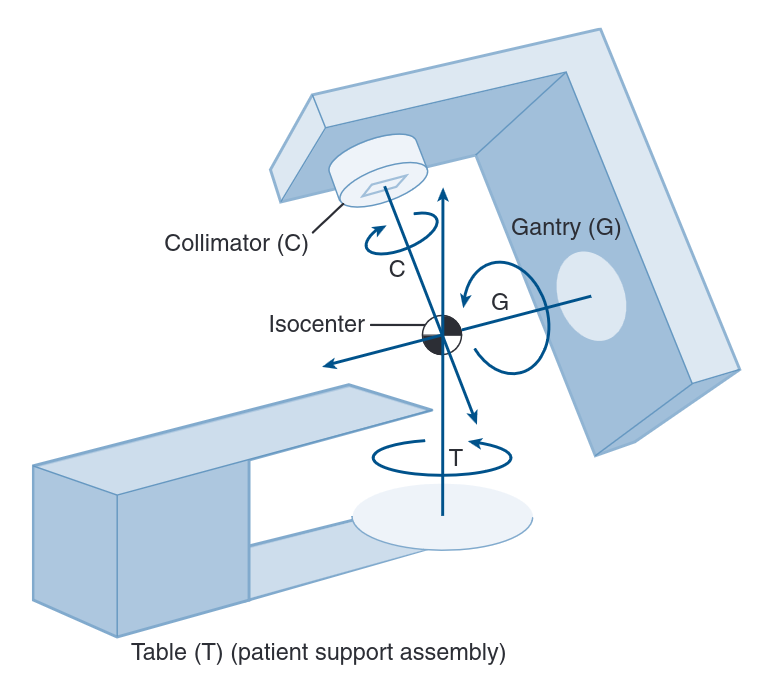
\includegraphics[width=0.5\textwidth]{Content/Images/linac.png}
    \caption{Layout of gantry-based linac \cite{abeloff_clinical_oncology}}
    \label{fig:linacLayout}
\end{figure}

\subsubsection{Multileaf collimator (MLC)}

A \emph{multileaf collimator} (MLC) is a collimator composed of individual leaves of a high atomic number material, typically tungsten. These leaves can move independently in and out of the path of a beam to shape and vary its intensity, to enable generating beams of particles with high precision, covering the exact geometry of the targeted body area. \cite{abeloff_clinical_oncology}

\begin{figure}[H]
    \centering
    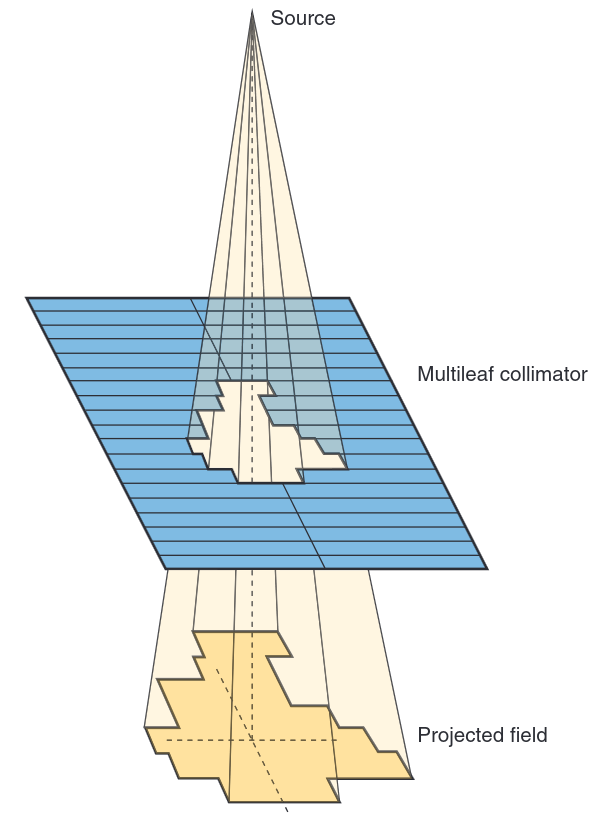
\includegraphics[width=0.5\textwidth]{Content/Images/mlc.png}
    \caption{Narrowing beam with multileaf collimator \cite{abeloff_clinical_oncology}}
\end{figure}

\subsection{DICOM}

\emph{Digital Imaging and Communications in Medicine} (DICOM) is a technical standard for the digital storage, management and transmission of medical images and related information. It is important to notice that this standard specifies not only file format but also information like the set of protocols used for communication and syntax of commands and associated information that can be exchanged using these protocols. \cite{DICOM_spec_intro}

\subsubsection{DICOM file format}

A DICOM data consists of various attributes and is grouped into data sets. This ensures that all relevant data about the image (like patient ID) cannot be separated and accidentally lost. Besides attributes like patient name, age etc. file contains one special attribute - image pixel data. Pixel data can be converted to other formats like JPEG or PNG and the easily displayed on any modern device. \cite{DICOM_spec_file}

\section{Artificial Intelligence}

\emph{Artificial intelligence} (AI) is a very broad term that generally describes any form of intelligent behaviour displayed by a computer system. AI is a field of research in computer science that explores approaches that enable machines to observe reality, learn and take intelligent actions to achieve defined goals.

There are numerous subfields of AI, concentrated around particular goals, like reasoning, natural language processing or support for robotics. Current research focuses on the achievement of artificial general intelligence, for example, the ability to perform any task that a human can perform, at least at an equal level, but such a state has not yet been achieved. Therefore, any current tool or model focuses on solving a specific task.

Simulating intelligence boils down to separating problems into several subproblems that can be addressed individually using different tools and models. The following system characteristics are not exhaustive examples of possible research fields:

\begin{itemize}
    \item Reasoning and problem-solving
    \item Knowledge representation
    \item Planning and decision-making
    \item Learning
    \item Natural language processing
    \item Perception
    \item Social intelligence
\end{itemize}

This thesis will focus on one of them - perception. It describes the ability to process input from various sensors (like sonar, wireless signals, cameras, microphones, radar or lidar) to deduce aspects of the world. This field includes topics like object recognition and tracking, facial recognition, speech recognition and image classification. The branch that deals with research in this area is called \emph{computer vision}. \cite{russell_norvig_2020}

\subsection{Computer Vision}

\emph{Computer vision} tasks involve processing, analyzing and extracting data from the real world in the form of visual input to produce symbolic or numerical information, often in the form of decisions. \cite{klette_2014}

For a CV algorithm to analyze an image, it must first be processed into a form that is suitable for the algorithm. This frequently involves the extraction of specific features from the given image, such as edges, whose analysis will lead to meaningful conclusions.

\section{Tools of image processing and analysis}

\emph{Digital image} is image composed of picture elements, called \emph{pixels}. In this case, each pixel represents a two-dimensional function with spatial coordinates given by $x$ and $y$ as input and a finite, discrete numerical representation of its intensity or grey level as output. \cite{digital_image_processing}

\subsubsection{Color representation and greyscale}

A \emph{greyscale} image consists of pixels that have only one value representing the amount of light, and therefore only contains intensity information. \cite{digital_photography} On the other hand in \emph{coloured} images one pixel can store more values called \emph{channels}, each representing one of the colour components that combined produce the desired colour. A grayscale image has just one channel.

In the code, greyscale images can therefore be represented as a two-dimensional array of $n \times m$ numbers and colour images as a three-dimensional array of $n \times m \times c$ numbers, where $n$ and $m$ specify the dimension of the image and $c$ represents the number of channels.

\subsubsection{RGB}

The \emph{RGB colour model} is an additive model which enables the representation of a wide range of colours by adding together \emph{red}, \emph{green} and \emph{blue} - primary colours of light. The name of the model comes from the first letters of its component colours. \cite{colour_photography}

\subsection{Thresholding (binarisation)}

Image \emph{thresholding} is a method of segmenting images. It involves modifying the image so that each pixel has one of two values often interpreted as the presence or absence of an object. For this reason, thresholding is also called \emph{binarisation}. Simple binarisation methods consist of replacing each pixel in the image with a black pixel if the pixel intensity is less than a fixed threshold $T$, or with a white pixel if the pixel intensity is greater than $T$.\cite{morphology_book} 

Binarisation can only be performed on a monochannel image. Multichannel images must first be converted to monochannel ones. Another approach would be to apply binarisation to each channel separately and then combine the image. One of the methods is to leave a white pixel if its value in each channel is above the threshold.

Binarisation helps to significantly reduce the dimensionality of the problem and is the basis for many further image analysis methods. 

\subsubsection{Adaptive thresholding}

Simple methods use global value as a threshold. However, this is not always advantageous; for example, if an image contains uneven lighting in different areas, it can cause dimmed areas to turn all black, leaving the desired features undetected. 

The solution is \emph{adaptive thresholding}, which determines the threshold value for a pixel based only on the region around it. As a result different thresholds for different regions of the image are used, giving better results for images with varying illumination. 

\begin{figure}[H]
    \centering
    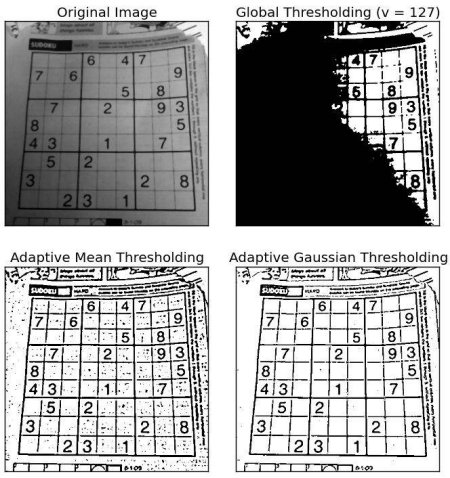
\includegraphics[width=0.6\textwidth]{Content/Images/adaptive_threshold.jpg}
    \caption{Comparison of global and adaptive thresholding for image with varying illumination \cite{adaptive_thresholding}}
\end{figure}

\subsection{Inversion}

Binary image \emph{inversion} is the process of transforming an image in such a way that the pixels that were originally black are transformed into white, and vice versa. For RGB images inverted image is a \emph{negative} of the original image. \cite{inversion_matlab} It is achieved by subtracting the value of the pixel from its maximum possible value for each channel:

\begin{equation}
    I'(x, y, c) = \mathbf{M} - I(x, y, c)
\end{equation}

where
\begin{itemize}
    \item $I'$ is the inverted image,
    \item $\mathbf{M}$ is max value that pixel can have
    \item $I(x, y, c)$ is value of original image for pixel's channel $c$ and coordinates $x$ and $y$
\end{itemize}

\begin{figure}[H]
    \centering
    \begin{subfigure}[b]{0.15\textwidth}
        
\includegraphics[width=\textwidth]{Content/Images/agh_logo_original.jpg}
    \end{subfigure}
    \begin{subfigure}[b]{0.15\textwidth}
        
\includegraphics[width=\textwidth]{Content/Images/agh_logo_inverted.png}
    \end{subfigure}
    \caption{Original and inverted image \cite{agh_logo}}
\end{figure}

\subsection{Filtering}

\emph{Filtering} is a process of transforming the image into a slightly modified version by sequentially applying a specifically designed image, called \emph{the kernel}, to all pixels of the source image. Depending on the choice of kernel, a different effect can be obtained. Filtering can be performed by convolution between the kernel and the image. \cite{digital_image_processing}


\subsubsection{Example filtering operations}

\begin{itemize}
    \item Edge detection
    \item Sharpening
    \item Blurring
    \item Identity
    \item Fourier lowpass/highpass (frequency filtering)
\end{itemize}

\subsubsection{Convolution}

\emph{Convolution} is fundamental \emph{neighbourhood image transformation}, meaning its output value at a given pixel is a function of the values of the pixels present in the neighbouring region centred on the considered pixel.

Convolution is defined as an operation on two images $f$ and $g$, whose origin is in the centre of its pixel frame $\mathcal{D}_g$ (middle one pixel). The output of the convolution at a given pixel $x$ of $f$ is defined by the weighted sum of the pixels of $f$ falling within $\mathcal{D}_g$ when the origin of $\mathcal{D}_g$ coincides with $\mathbf{x}$, the weights being defined by the values of $g$ \cite{morphology_book}:

\begin{equation}
    [f*g](\mathbf{x}) = \sum_{\mathbf{b} \in \mathcal{D}_g} [f(\mathbf{x} - \mathbf{b}) g (\mathbf{b})]
\end{equation}

Intuitively, convolution is the process of adding each element of the image to its local neighbours, weighted by the kernel.

\begin{figure}[H]
    \centering
    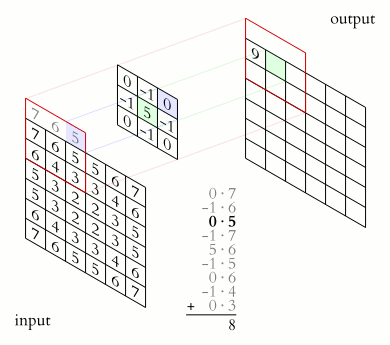
\includegraphics[width=0.6\textwidth]{Content/Images/2D_Convolution_Animation.png}
    \caption{Visualisation of 2D discrete convolution \cite{convolution_animation}}
\end{figure}

\subsection{Edge detection}

\emph{Edge detection} is a set of mathematical techniques that aim to identify \emph{edges}, defined as curves in a digital image where the brightness of the image changes sharply, or where there are discontinuities. Edge detection is an essential tool in image processing and computer vision, especially in area and feature extraction. The algorithms differ in their choice of kernel, called an \emph{operator}. \cite{Digital_Image_Processing_2}

\subsubsection{Sobel operator}

The operator uses two 3×3 kernels which are applied to the original image to calculate approximations of the derivatives – one for vertical changes, and one for horizontal. The resulting images are defined as follows: \cite{sobel_article}

\begin{equation}
    \mathbf{G}_x = 
    \begin{bmatrix}
        +1 & 0 & -1\\
        +2 & 0 & -2\\
        +1 & 0 & -1
    \end{bmatrix} * \mathbf{A}
\end{equation}

\begin{equation}
    \mathbf{G}_y = 
    \begin{bmatrix}
        +1 & +2 & +1\\
        0 & 0 & 0\\
        -1 & -2 & -1
    \end{bmatrix} * \mathbf{A}
\end{equation}

where
\begin{itemize}
    \item $\mathbf{A}$ is the source image;
    \item $\mathbf{G}_x$ image, where each point contains the horizontal derivative approximation
    \item $\mathbf{G}_y$ image, where each point contains the vertical derivative approximation
\end{itemize}

The x-coordinate increases in the 'right' direction and the y-coordinate increases in the 'down' direction. Resulting gradient approximations can be combined at any point in the image to produce a gradient magnitude:

\begin{equation}
    \mathbf{G} = \sqrt{\mathbf{G}_x^2 + \mathbf{G}_y^2}
    \label{eq:sobelGradientMagnitude}
\end{equation}

\subsubsection{Example images}

\begin{figure}[H]
    \centering
    \begin{subfigure}[b]{0.45\textwidth}
        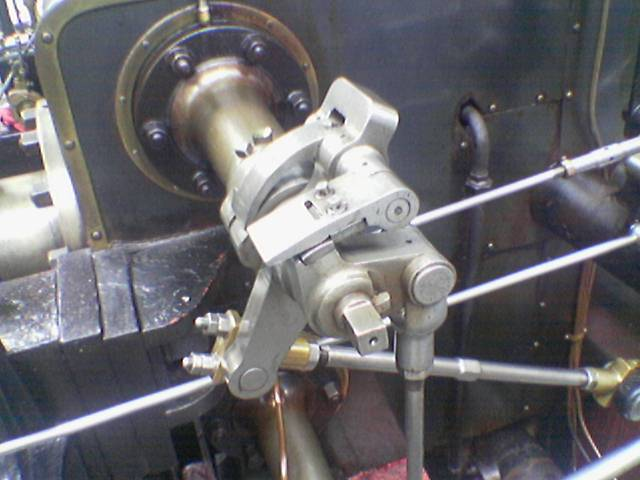
\includegraphics[width=\textwidth]{Content/Images/sobel_example_before.png}
    \end{subfigure}
    \begin{subfigure}[b]{0.45\textwidth}
        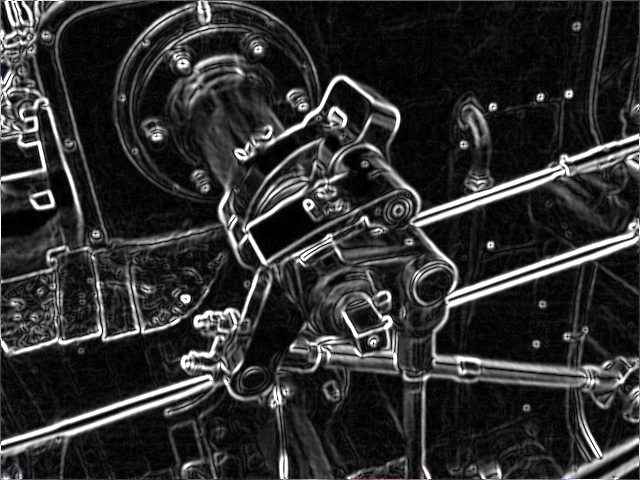
\includegraphics[width=\textwidth]{Content/Images/sobel_example_after.png}
    \end{subfigure}
    \caption{Original image \cite{sobel_example_before} and resulting image with combined gradient approximations computed with Sobel operator \cite{sobel_example_after}}
\end{figure}

\subsection{Blob detection}

\emph{Blob} is a group of pixels in an image that are connected and share common properties. \emph{Blob detection} is the process of detecting regions in an image that differ in properties, such as shape, colour, or brightness from its surroundings. The most common blob detection methods use convolution. The procedure typically involves three steps: 

\begin{enumerate}
    \item thresholding, which divides the image into segments,
    \item assembling linked pixels into clusters,
    \item examining clusters to find details such as their dimensions, centres and shapes. \cite{geeks_for_geeks_blob_detection}
\end{enumerate}



\subsection{Morphological operations}

\emph{Morphology} can be defined as a theory for the analysis of spatial structures. It aims at analysing the shape and form of objects. It can be used to solve such tasks as:

\begin{itemize}
    \item Noise filtering
    \item Correction of uneven illumination
    \item Edge enhancement
    \item Image segmentation
\end{itemize}

There are two basic operations: \emph{erosion} and \emph{dilation}, and their combinations \emph{opening} and \emph{closing}.

\subsubsection{Structuring Element (SE)}

The basic idea of morphology is to use a pre-defined shape to probe an image and then draw conclusions on how well or poorly this shape fits the other shapes in the image. The "probe" is called the \emph{structuring element} and it is a separate image (kernel) of smaller size and well-defined shape. In practice, in image analysis, the most common kernel will be the square matrix $ n \times n $.

\subsubsection{Erosion}

The erosion of a set $X$ by a structuring element $B$ is denoted by $\varepsilon_B(X)$ and is defined as the locus of points $\mathbf{x}$ such that $B$ is included in $X$ when its origin is placed at $\mathbf{x}$:

\begin{equation}
    \varepsilon_B(X) = \{ \mathbf{x} | B_\mathbf{x} \subseteq X \}.
\end{equation}

Intuitively, it can be understood as reducing objects' edge by the kernel going around it.

\begin{figure}[H]
    \centering
    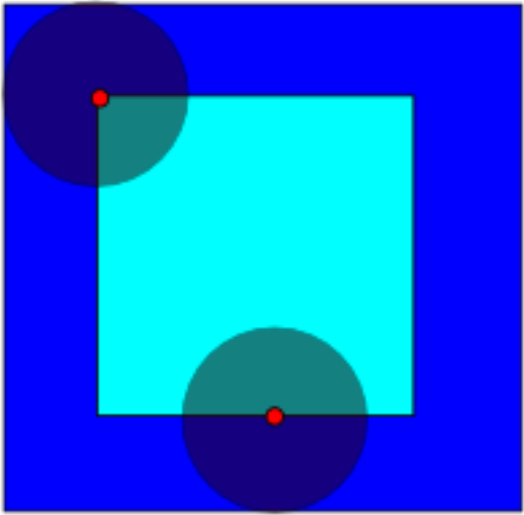
\includegraphics[width=0.25\textwidth]{Content/Images/Erosion.png}
    \caption{Erosion of dark-blue square by a circle structuring element \cite{erosion}}
\end{figure}

\subsubsection{Dilation}

The dilation of a set $X$ by a structuring element $B$ is denoted by $\delta_B(X)$ and is defined as the locus of points $\mathbf{x}$ such that $B$ hits $X$ when its origin coincides with $\mathbf{x}$:

\begin{equation}
    \delta_B(X) = \{ \mathbf{x} | B_\mathbf{x} \cap X \neq \emptyset \}.
\end{equation}

Intuitively, it can be understood as the thickening of an object by an edge caused by the kernel going around it.

\begin{figure}[H]
    \centering
    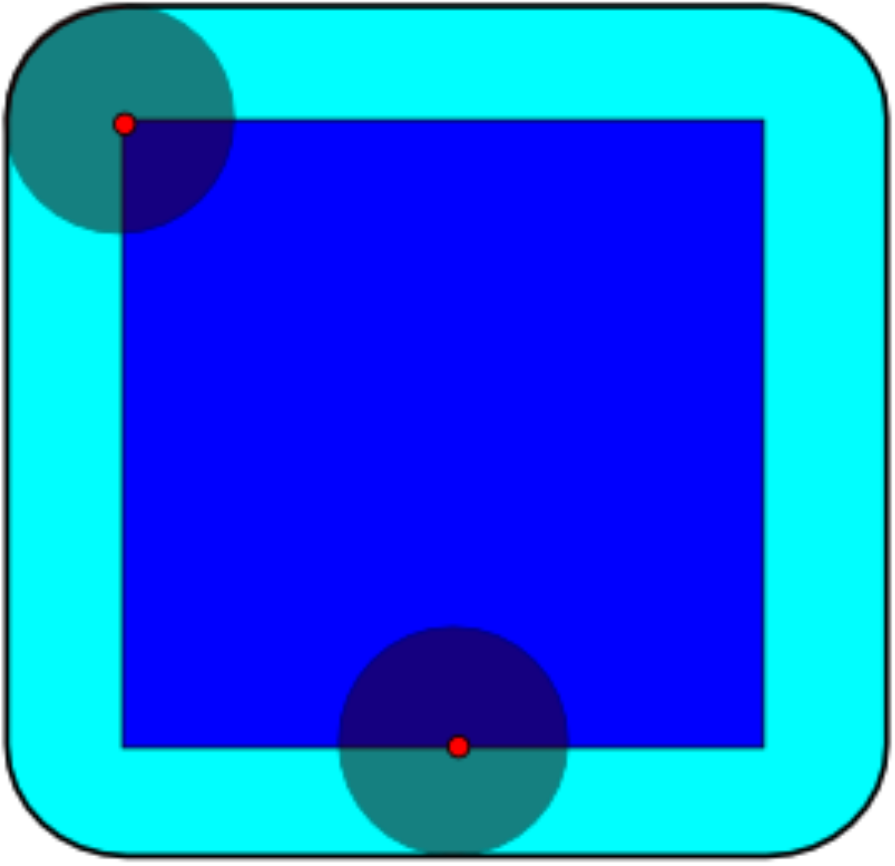
\includegraphics[width=0.25\textwidth]{Content/Images/Dilation.png}
    \caption{Dilation of dark-blue square by a circle structuring element \cite{dilation}}
\end{figure}

\subsubsection{Opening}

The opening $\gamma$ of an image $f$ by a structuring element $B$ is denoted by $\gamma_B(f)$ and is defined as the erosion of $f$ by $B$ followed by the dilation with the reflected SE $\check{B}$:

\begin{equation}
    \gamma_B(f) = \delta_{\check{B}} [ \varepsilon_B(f) ],
\end{equation}

which can also be written as:

\begin{equation}
    \gamma_B(X) = \bigcup\limits_{\mathbf{x}} \{ B_\mathbf{x} | B_\mathbf{x} \subseteq X \}
\end{equation}

\subsubsection{Closing}

The closing of an image $f$ by a structuring element $B$ is denoted by $\phi_B(f)$ and is defined as the dilation of $f$ with a structuring element $B$ followed by the erosion with the reflected SE $\check{B}$:

\begin{equation}
    \phi_B(f) = \varepsilon_{\check{B}} [ \delta_B(f) ],
\end{equation}

which can also be written as:

\begin{equation}
    \phi_B(X) = \bigcap\limits_{\mathbf{x}} \{ B_\mathbf{x}^c | X \subseteq B_\mathbf{x}^c \}
\end{equation}

Morphology description and definitions based on \cite{morphology_book}.

\begin{figure}[H]
    \centering
    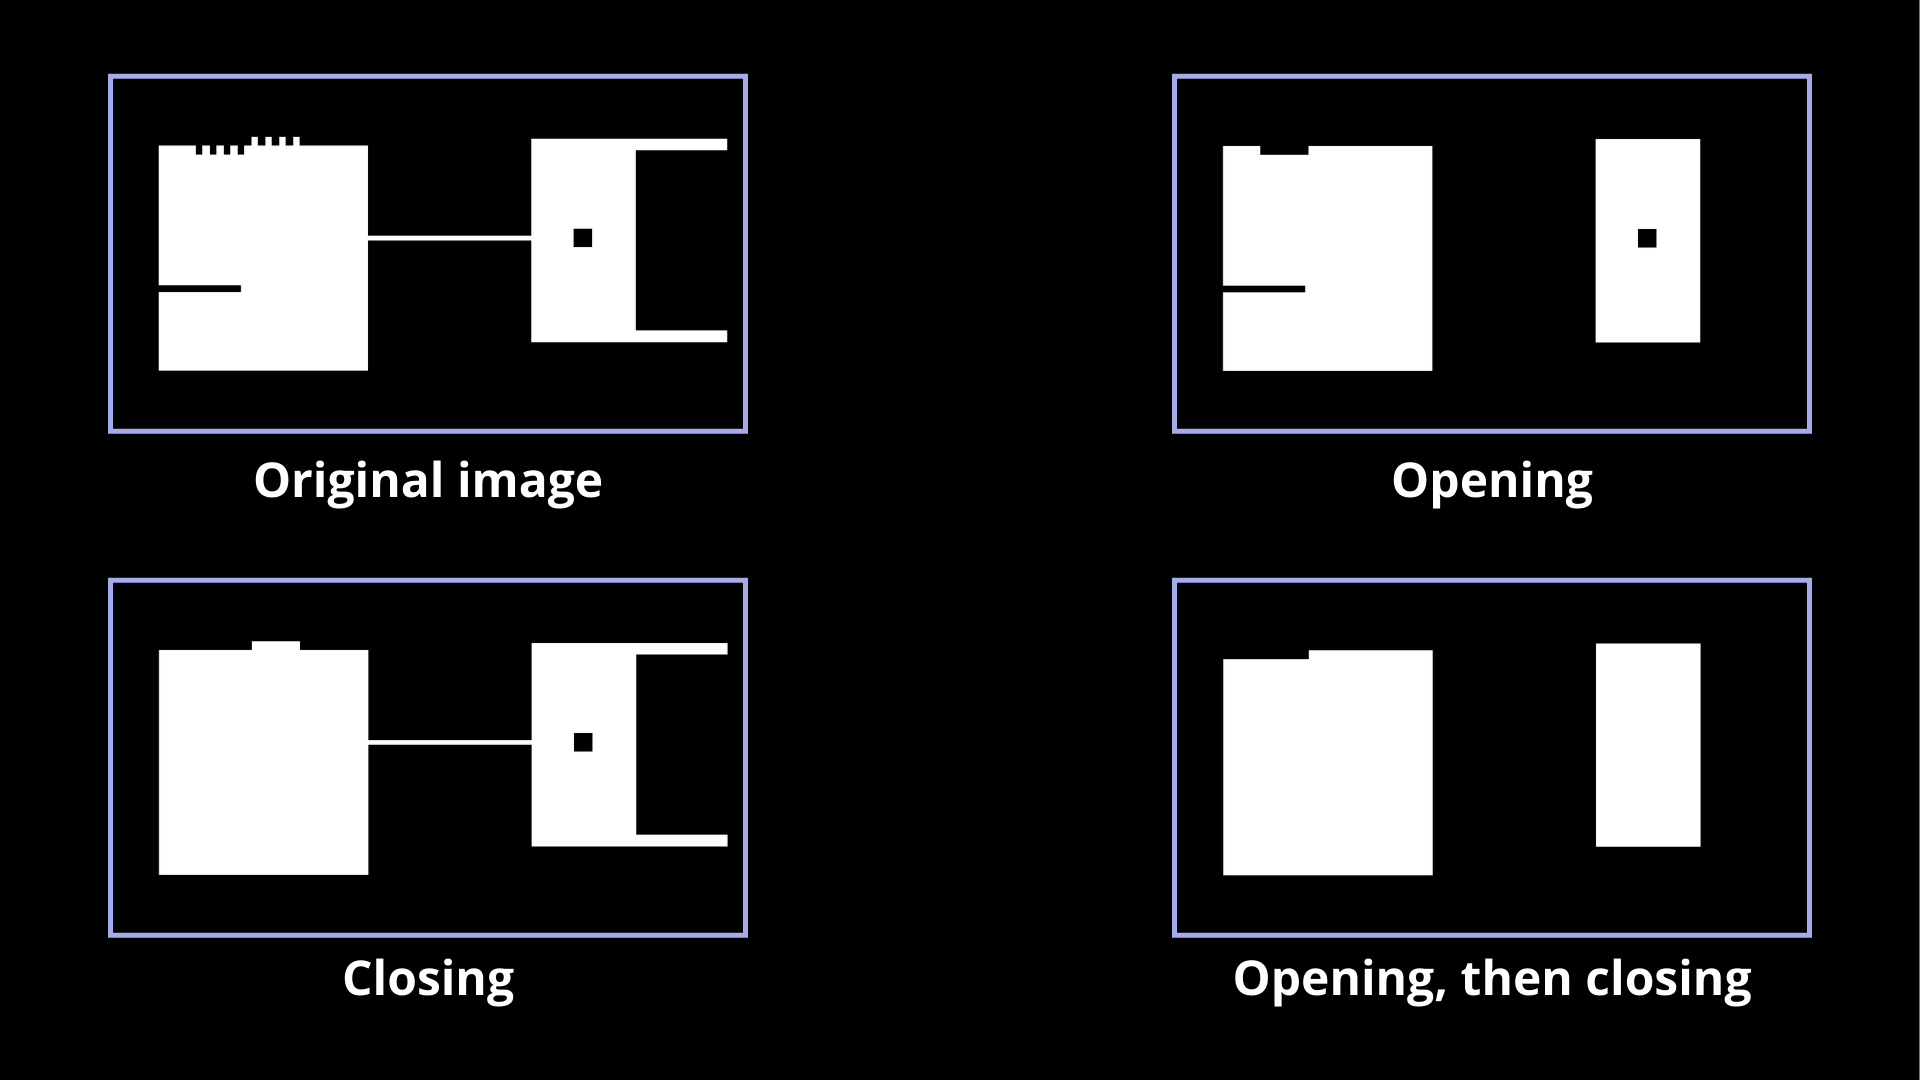
\includegraphics[width=0.8\textwidth]{Content/Images/opening_closing.png}
    \caption{Example of closing and opening operations}
\end{figure}

\section{Quality Control}

Linacs, like any advanced medical device, need constant maintenance and calibration. The whole process of taking care of the device's performance is called \emph{quality control} (QC).

One of the QC procedures for linacs is the \emph{Winston-Lutz test} (W-L test). The test aims to control the mutual alignment of the mechanical isocenter of linac (the point where the gantry axis and couch axis intersect) designated using treatment room laser system and actual radiation beam isocenter.

To conduct the test, a series of images must be taken in a specifically prepared environment. Then, images are analysed to conclude the position of the radiation isocenter. \cite{wl_og} \cite{wl_2}


\paragraph{}
Another QC procedure that can be performed is the \emph{leaves alignment analysis} (LA analysis) for MLCs. This procedure involves comparing the image taken, with the planned layout of leaves. If the detected area differs from the planned one, this means that the leaves are not aligning correctly, leading to erroneous generation of the radiation field by the linacs.

\paragraph{}
The environment setup and the process of capturing images are further explained in \autoref{chr:envSetup}. Image analysis procedure and description of algorithms can be found in \autoref{chr:wlTest} - for W-L test, and in \autoref{chr:laModule} - for LA analysis.

\section{Web applications}

An application that runs in a browser is a \emph{web application}. It is a very popular type of software considering its ease of use and portability for the average user and will continue to grow in future. \cite{future_of_web_apps_2024}

\subsection{Benefits of web apps}

Web applications have several benefits that make them a good choice for modern software development. The following section outlines some of the most significant ones.

\subsubsection{Accessibility}

Web apps can be accessed from any device that has access to a modern browser. People from different locations can access shared documents, files and other data, work on them synchronously and see changes made by others in real-time, without the need to exchange any additional data.

\subsubsection{Efficient development}

The process of developing an app is relatively simple. There is no need to manage the distribution of the application - if a new version is deployed, every user can use it instantly. Additionally, since any version can work on any modern browser, there is no need to maintain different iterations of the product significantly reducing the resources needed for its maintenance.

\subsubsection{Simplicity for users}

Users are not required to download apps and no additional software is required to be installed on the user's machine, which makes them easy to access and eliminates the need for user maintenance. Web apps are always up to date since they automatically receive security and software updates.

\subsubsection{Scalability}

Adding new capacity, like users or available space is easy, especially if data is stored in the cloud. There is no need to install or change any existing infrastructure. \cite{aws_web_app}

\subsection{Architecture of web applications}

Web apps have a \emph{client-server architecture}. The codebase is divided into two components - \emph{client-side} and \emph{server-side}.

\subsubsection{Client-side architecture}

Client-side scripts and data are loaded when a user visits the address of a web page in his browser. This is part of the application that displays data and provides interactive interface functionality (like buttons and forms) for the user. For this reason, it is often referred to as application \emph{frontend}.

When a user clicks on a button or link in the interface, the web browser loads and launches a script that reacts to this action rendering some page element, called \emph{component}, or communicating with the server-side of the application. 

\subsubsection{Server-side architecture}

Server-side code manages data processing and persistence. Users cannot directly interact with server-side functionality, only through the frontend interface. Therefore this part of the application is often called \emph{backend}. The backend often uses databases to store data and communicate with other servers to process complex data. \cite{aws_web_app}

\subsection{User Interface (UI)}

\emph{User interface} is the point of contact for interaction and communication between humans and electronic devices. This can include display screens, keyboards, mice, and the appearance of a desktop. It also refers to the way a user interacts with buttons, animations, sounds, typefaces, and other visual and audio components on a website or application. \cite{what_is_ui}

\subsection{Communication between frontend and backend}

There are many different ways and protocols in which the frontend and backend can communicate, but one of the most popular is the \emph{RESTful API}.

\emph{Application Programming Interface (API)} is a mechanism that enables two different software components to communicate with each other using a set of protocols and definitions.

REST is built on top of Hypertext Transfer Protocol (HTTP) and enables programmers to define a set of operations that can be performed on resources.

The resource is any data or content, that exists on the server. Resources are uniquely identified by a predefined address. This address of resource is called \emph{endpoint}.

The most common operations are: 

\begin{enumerate}

    \item POST

    Used to create previously non-existing resources.

    \item GET

    Used to read data of resource.

    \item PUT

    Used to update existing resources.

    \item DELETE

    Used to delete existing resources.

\end{enumerate}

Communication is based on the request-response cycle. The client sends a request to the server, server processes this request and sends back the response. All calls are stateless, which means that RESTful service cannot retain anything between calls. Data persistence is achieved with the usage of external databases. \cite{restful_api}

\subsection{Open source software}

In contrast to closed source, commercial software, \emph{open source software} is released under a license that gives users the right to use, change and distribute the software and its source code to anyone for any purpose. The important thing is that users get insight into the project's source code, which they can change and redistribute in other projects. \cite{open_source}

The development of this kind of application in a scientific environment is very important. Rather than providing a closed system that can process data on a one-time basis (often for a fee), developers are offering a comprehensive tool that can be reused in a range of other applications.
